\documentclass{llncs} %
\bibliographystyle{splncs}
\usepackage{url}
\usepackage{graphicx}
\usepackage{caption}

\newcommand{\source}[1]{\hfill Source: {#1} }

\begin{document}

\title{Supporting Meditative Awareness through Neurofeedback Wearables}
\author{Vincenzo Pace}
\institute{Karlruhe Institute of Technology, Karlsruhe, Germany}
\maketitle
\newpage
\section{Introduction}
Adoption and functionality of wearable devices are increasing and expected to continue to do so \cite{Patel}. In the west, meditation is accepted more widely as a means of health improvement \cite{Tang:et al}.
Consumer EEG devices and freely available EEG/ERP databases \cite{ucsd} offer a chance to use algorithms to analyze a user's meditation experience and provide feedback for improvement.
This work presents the current state of art of consumer EEG devices, the signals involved in meditation and the possibility for usage of such devices for meditation training.
In the end, three popular EEG headsets will be compared and evaluated.
\subsection{EEG}
EEG stands for electroencephalography and is a process to record the electrical activity in the brain. The measured signal are voltage changes in and between neurons. EEG can only measure measure signal in the outer regions of the brain \cite{Sitaram}.
The brains signal is in the order of mikrovolt \cite{Berger}.  For measurement, EEG electrodes are placed on the test subjects scalp. In Research, up to 256 electrodes are used \cite{Seeck}, while consumer grade devices use around 10\% of this. \cite{Maskeliunas}
The electrical signal is measured as frequencies and go through an EEG ampflifier. These get passed to a Fast Fourier Transformation (FTT) or wavelet transformation \cite{Akin} to produce distinct waves, which are then categorized according to known patterns \cite{Shaker}.
Brain waves of individuals can be compared to aggravated data of many test subjects, to search for disorders \cite{Loo} or match for meditation success \cite{Tang:et al}, access to enough datapoints assumed.
There are four main brain frequencies \cite{Cahn}:
% quantitative eeg 
\begin{itemize}
    \item 
    Beta Waves (frequency range from 14 Hz to about 30 Hz), associated with intellectual activity and outwardly focused concentration
    \item 
    Alpha Waves (frequency range from 7 Hz to 13 Hz), associated with relaxation
    \item 
    Theta Waves (frequency range from 4 Hz to 7 Hz), associated with mental inefficiency \cite{Hammond}, zone between wake and sleep
    \item 
    Delta Waves (frequency range up to 4 Hz), associated with sleeping, learning disabilities \cite{Hammond}
\end{itemize}
From the data, conclusions about attention \cite{Berka}, stress \cite{Hosseini}, cognitive load \cite{Antonenko} and more are possible.
While EEG caps are usually used in research and academia \cite{Seeck}, headsets provide a reasonable solution for consumers with less complexity, but also lower precision\cite{Maskeliunas}.
For the accuracy of the measurement it is still crucial, that the sensors are correctly affixed \cite{Seeck}, so that they measure the brain regions that are involved in meditation.

EEG devices are either gel based or dry. In Research, gel electrodes are used and cost thousands of dollars, have wired signal transmission and are time consuming to setup and are uncomfortable to wear.
Consumer devices on the other hand are dry, wireless and cost only a few hundreds of dollars. \cite{Decho}
\subsection{Neurofeedback}
Neurofeedback (NFB), also called EEG biofeedback, is a therapy that was invented as a method for training brainwave patterns through operant conditioning and is known since the 1960s \cite{Hammond}. %OK like that?
It is used not only as a treatment of disorders, but also in peak performance training. NFB experiments led to the deleopment of the field of brain-machine interfaces \cite{Sitaram}.
Operant conditioning is the learning process where a behavior is modified by punishment or reward, the famous example being Pavlov's dog \cite{Spence}. NFB never uses punishment though. In NFB, the neural activity is recorded and presented to the participant in real time.  
Usually people are not aware of their brain waves, so seeing them on a screen helps by giving you the ability to influence them. This is the operant conditioning part. In the beginning, the changes are only short-lived, but with practice can become lasting. 

\begin{figure}
    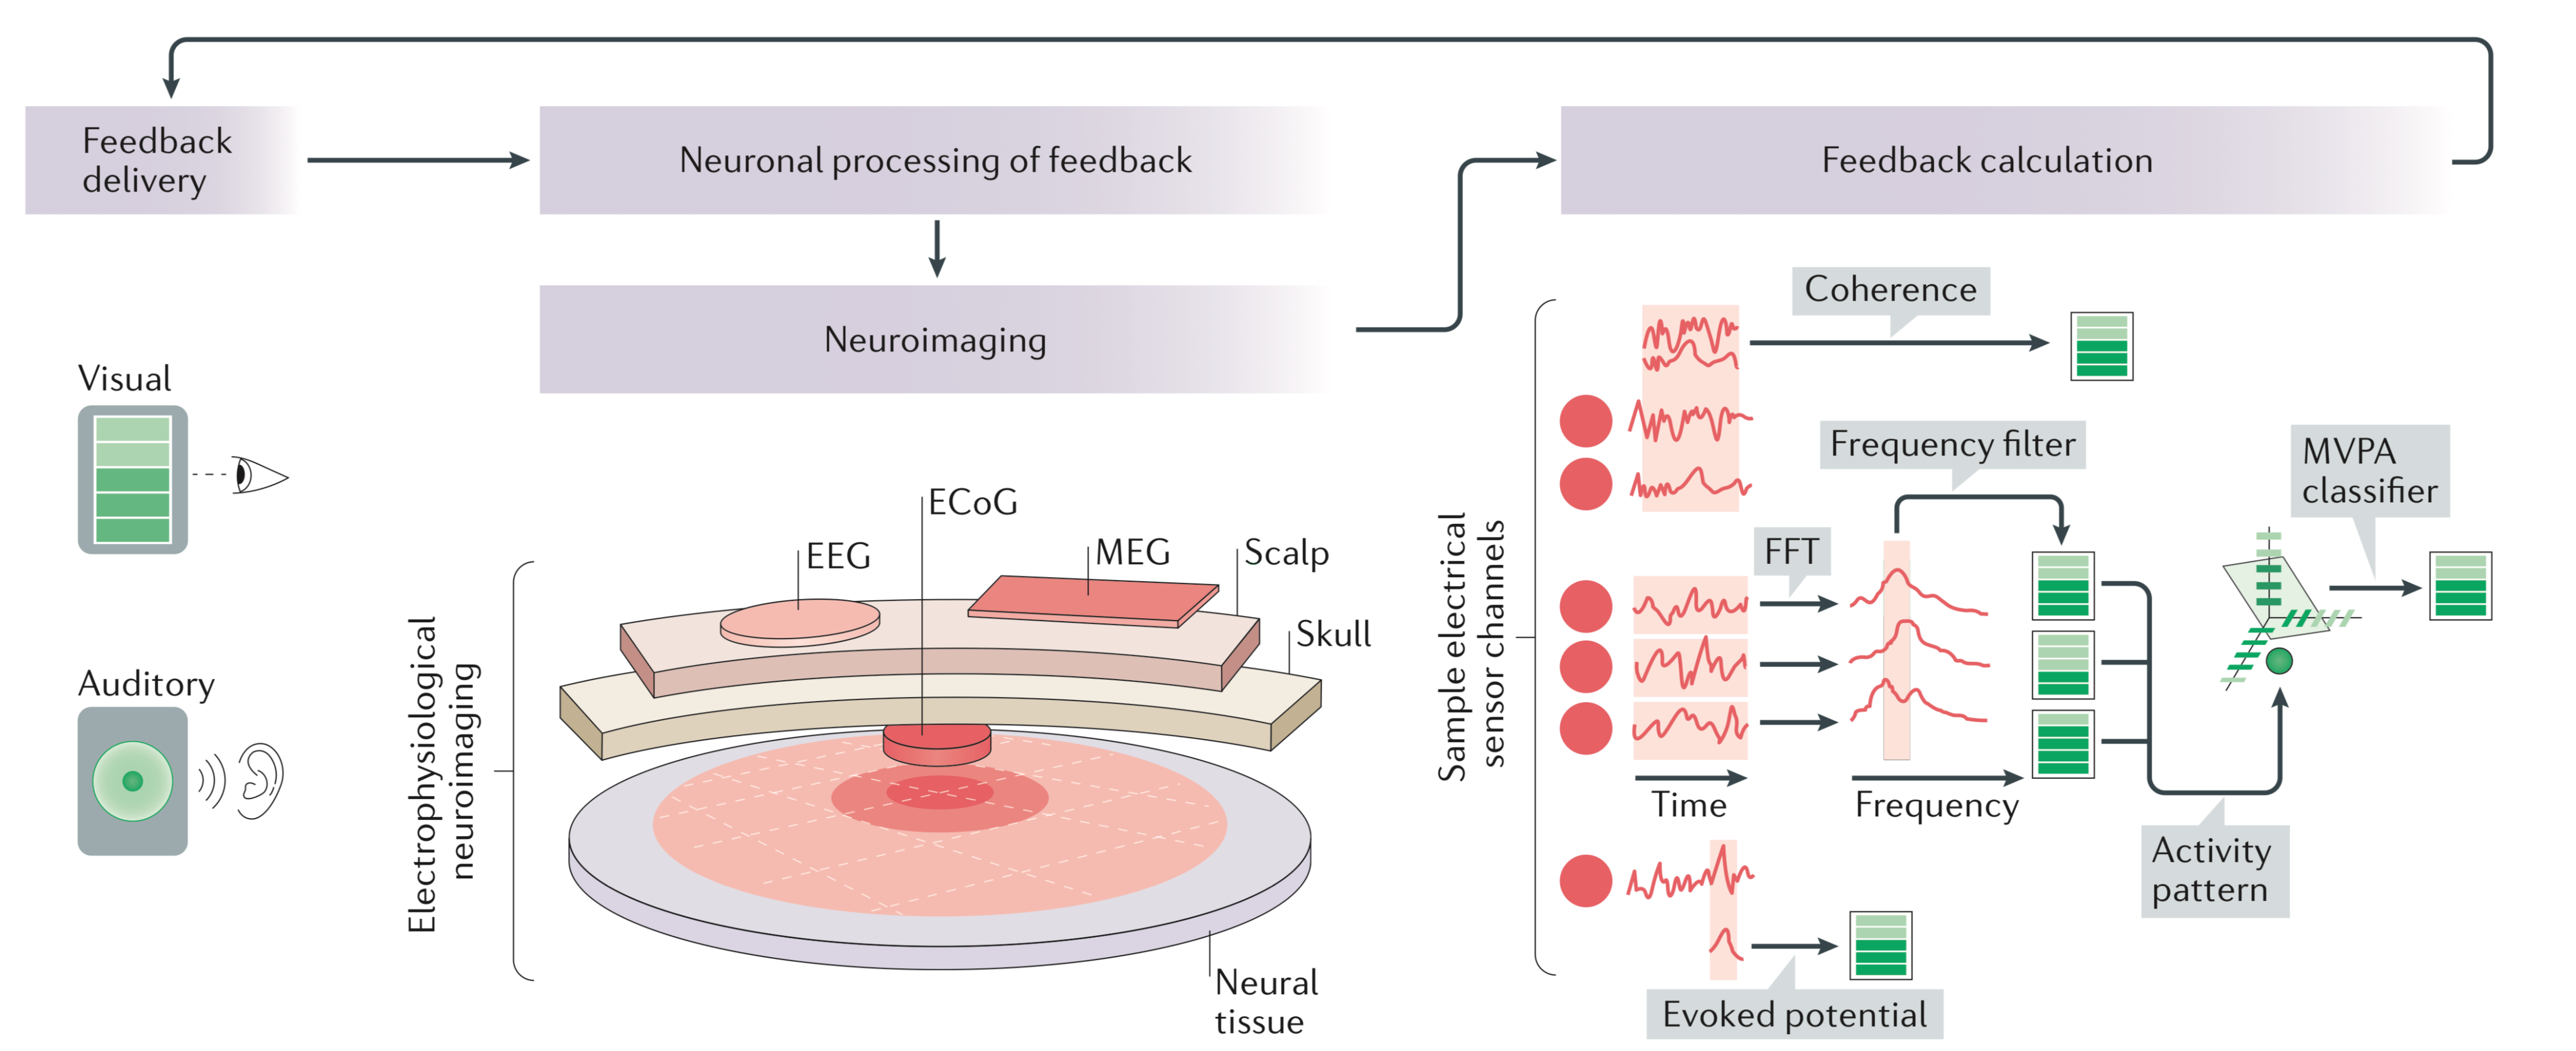
\includegraphics[width=\linewidth]{Neurofeedback.png}
    \caption{The neurofeedback process}  \label{neurofeedback}
    \source{Sitaram et al, 2016}
\end{figure}

NFB is non-invasive and is sometimes used as an alternative to medication \cite{Hammond}. Another unique kind of NFB is called LENS, where a tiny electromagnetic signal is introduced to the electrodes and transported to the brain.
However, it is not recommended to use NFB equipment without any expertise. Also, the training should be individualised to the unique brainwave patterns of each person. A physician should always be consulted first.
Otherwise, negative side effects or degradation of existing disorders are possible. Only healthy individuals should use a NFB device for meditation training on their own risk.

\subsection{Meditation}
Over the last decades, meditation has gained the interest of popular culture and the scientific community.
Documented beneficial effects range from mood improvements to structural changes \cite{Davidson} in various regions of the brain, such as the amygdala (responsible for stress and anxiety), anterior cingulate cortex, brain stem (breathing)
and the default mode network \cite{Tang:et al}.
Therefore, meditation has become part of psychiatric interventions \cite{Hoelzel}, high performance sports and personal development.
% QUOTE
Historically, meditation stems from buddhist practices and has been part of eastern culture for centuries, though variations were also practiced by the ancient greeks \cite{Hadot:Davidson}.

Though there is not one single meditation practice, the methods are plentiful. While often associated with stillness and watching ones breath,
there are also more active forms of meditation that involve more movement. Travis and Shear categorize meditation practices into focused attention, open monitoring and automatic self-transcending.\cite{Travis} 
Since this categorization is based on different EEG patterns and would be part of the wearable device, I will follow this categorization and differentiate where appropriate.

All these potential benefits lead to an increasing populace that wants to learn and practice meditation, so that a device that helps in the acquisition of this skill becomes desirable. 
The demands, functions, challenges and applications for such a device are the topic of this work.
\subsection{Awareness}
Mindfulness and awareness are two terms often mentioned in the context of meditation and there is no exact, agreed upon scientific definition to separate these two.
\section{Goals}
Since the beneficial effects of meditation are so various, the potential goals of using a wearable device 
that provides neurofeedback to its user are inherently diverse. Machine assisted meditation could help individuals to 
improve faster, track their progresssion, analyze the state of mind and lower the entrance barrier for novel practicioners. \cite{brand:del} \

The differences in EEG signals induced by the different meditation practices enable a categorization
and dedicated training regime to offer the device and software solution to a wider audience. \cite{Travis}
\section{Measurement Data}
\subsection{Biological Signals}
\begin{itemize}
    \item EEG
    \item brain blood flow infrared spectroscopy
\end{itemize}
Combination of NIRS and EEG would be optimal! There is no such device yet for consumers though.
Possible?

\subsection{Measuring}
\subsection{Challenges}
Such a QEEG Assesment usually takes about 1.5 hours, which is too long for a consumer.
Involuntary movement of the tongue, eyeballs, jaw and facial muscles produce noise in the milivolt range, while brain signals are on 
the order of mikrovolt. These artifacts do not only occur in consumer great EEG devices, but also in medical grade.
These artifacts need to be filtered out to produce a reliable signal for further analysis \cite{Bashivan: et al}, which will be extremely difficult, since the device would need to know when a person moved ever so slightly \cite{Hammond}.

The time window of measurement is also crucial for the accuracy of machine learning models.
\subsection{Processing and evaluation}
\cite{Lotte}
\section{Training procedure}
\section{Available Devices}
\subsection{Neurosky - Mindwave Mobile 2}
\subsection{InteraXon Inc. - Muse 2}
\subsection{Emotiv - Epoc+}
\section{Conclusion}


\begin{thebibliography}{[MT1]}
    \bibitem{brand:del}
    Tracy Brandmeyer, Arnaud Delorme,
    Meditation and neurofeedback
    Frontiers in Psychology, Article 688 (October 2013).
    \bibitem{Tang:et al}
    Tang, Yi-Yuan, Britta K. Hölzel, and Michael I. Posner. "The neuroscience of mindfulness meditation." Nature Reviews Neuroscience 16.4 (2015): 213-225.
    \bibitem{Bashivan: et al}
    Bashivan, Pouya, Irina Rish, and Steve Heisig. "Mental state recognition via wearable EEG." arXiv preprint arXiv:1602.00985 (2016).    
    \bibitem{Travis} 
    Travis, Fred, and Jonathan Shear. "Focused attention, open monitoring and automatic self-transcending: categories to organize meditations from Vedic, Buddhist and Chinese traditions." Consciousness and cognition 19.4 (2010): 1110-1118.
    \bibitem{Hoelzel}
    Hölzel, Britta K., et al. "How does mindfulness meditation work? Proposing mechanisms of action from a conceptual and neural perspective." Perspectives on psychological science 6.6 (2011): 537-559.
    \bibitem{Cahn}
    Cahn, B. Rael, and John Polich. "Meditation states and traits: EEG, ERP, and neuroimaging studies." Psychological bulletin 132.2 (2006): 180.
    \bibitem{Braboszcz}
    Braboszcz, Claire, and Arnaud Delorme. "Lost in thoughts: neural markers of low alertness during mind wandering." Neuroimage 54.4 (2011): 3040-3047.
    \bibitem{Zoefel} 
    Zoefel, Benedikt, René J. Huster, and Christoph S. Herrmann. "Neurofeedback training of the upper alpha frequency band in EEG improves cognitive performance." Neuroimage 54.2 (2011): 1427-1431.
    \bibitem{Berger}
    Berger, Hans. "Über das elektrenkephalogramm des menschen." European archives of psychiatry and clinical neuroscience 87.1 (1929): 527-570.
    \bibitem{Seeck}
    Seeck, Margitta, et al. "The standardized EEG electrode array of the IFCN." Clinical Neurophysiology 128.10 (2017): 2070-2077.
    \bibitem{Maskeliunas}
    Maskeliunas, Rytis, et al. "Consumer-grade EEG devices: are they usable for control tasks?." PeerJ 4 (2016): e1746.
    \bibitem{Surangsrirat}
    Surangsrirat, Decho, and Apichart Intarapanich. "Analysis of the meditation brainwave from consumer EEG device." SoutheastCon 2015. IEEE, 2015.
    \bibitem{Akin}
    Akin, Mehmet. "Comparison of wavelet transform and FFT methods in the analysis of EEG signals." Journal of medical systems 26.3 (2002): 241-247.
    \bibitem{Shaker}
    Shaker, Maan M. "EEG waves classifier using wavelet transform and Fourier transform." brain 2 (2006): 3.
    \bibitem{Lotte}
    Lotte, Fabien, et al. "A review of classification algorithms for EEG-based brain–computer interfaces." Journal of neural engineering 4.2 (2007): R1.
    \bibitem{Antonenko}
    Antonenko, Pavlo, et al. "Using electroencephalography to measure cognitive load." Educational Psychology Review 22.4 (2010): 425-438.
    \bibitem{Berka}
    Berka, Chris, et al. "Real-time analysis of EEG indexes of alertness, cognition, and memory acquired with a wireless EEG headset." International Journal of Human-Computer Interaction 17.2 (2004): 151-170.
    \bibitem{Hosseini}
    Hosseini, Seyyed Abed, and Mohammad Ali Khalilzadeh. "Emotional stress recognition system using EEG and psychophysiological signals: Using new labelling process of EEG signals in emotional stress state." 2010 international conference on biomedical engineering and computer science. IEEE, 2010.
    \bibitem{Loo}
    Loo SK, Barkley RA. Clinical utility of EEG in attention deficit hyperactivity disorder. Appl Neuropsychol 2005; 12(2): 64-76.
    \bibitem{Davidson}
    Davidson, Richard J., and Antoine Lutz. "Buddha's brain: Neuroplasticity and meditation [in the spotlight]." IEEE signal processing magazine 25.1 (2008): 176-174.
    \bibitem{Decho}
    Surangsrirat, Decho, and Apichart Intarapanich. "Analysis of the meditation brainwave from consumer EEG device." SoutheastCon 2015. IEEE, 2015.
    \bibitem{Hadot:Davidson}
    Hadot, Pierre; Arnold I. Davidson (1995) Philosophy as a Way of Life: Spiritual Exercises from Socrates to Foucault ISBN 0-631-18033-8 pages 83-84
    \bibitem{Patel}
    Patel, Mitesh S., David A. Asch, and Kevin G. Volpp. "Wearable devices as facilitators, not drivers, of health behavior change." Jama 313.5 (2015): 459-460.
    \bibitem{ucsd}
    \url{https://sccn.ucsd.edu/~arno/fam2data/publicly_available_EEG_data.html}
    \bibitem{Seo}
    Seo, Ssang-Hee, and Jung-Tae Lee. "Stress and EEG." Convergence and hybrid information technologies. IntechOpen, 2010.
    \bibitem{Hammond}
    Hammond, D. Corydon. "What is neurofeedback?." Journal of neurotherapy 10.4 (2007): 25-36.
    \bibitem{Sulzer}
    Sulzer, James, et al. "Real-time fMRI neurofeedback: progress and challenges." Neuroimage 76 (2013): 386-399.
    \bibitem{Spence}
    Spence, Kenneth Wartenbee. Behavior theory and conditioning. Vol. 35. New Haven: yale university Press, 1956.
    \bibitem{Sitaram}
    Sitaram, Ranganatha, et al. "Closed-loop brain training: the science of neurofeedback." Nature Reviews Neuroscience 18.2 (2017): 86.
\end{thebibliography}
\end{document}